% 4-Bit-Ripple-Carry-Addierer: Stufe 0 = Halbaddierer, Stufen 1-3 = Volladdierer.
% Optional vor \input setzen (sonst symbolische Beschriftung):
%   \def\RCAinput#1#2{...}  Beschriftung des Eingangs a_i/b_i, #1 = a/b, #2 = Stufe
%   \def\RCAcarry#1{...}    Beschriftung des Übertrags c_#1
%   \def\RCAsum#1{...}      Beschriftung des Summenbits s_#1
\providecommand{\RCAinput}[2]{$#1_{#2}$}
\providecommand{\RCAcarry}[1]{$c_{#1}$}
\providecommand{\RCAsum}[1]{$s_{#1}$}
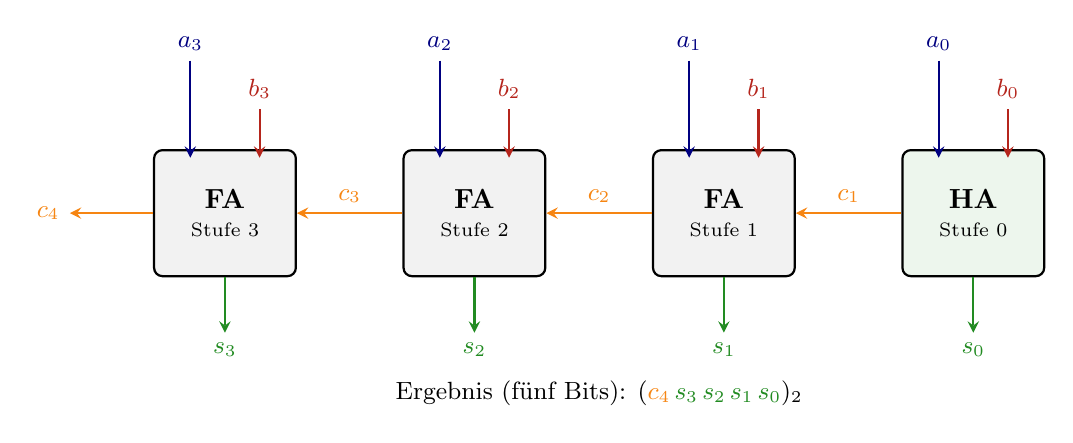
\begin{tikzpicture}[
    scale=0.88, >=stealth,
    fa/.style={draw, thick, fill=gray!10, rounded corners=3pt, minimum width=1.8cm, minimum height=1.6cm, align=center},
    ha/.style={fa, fill=ForestGreen!8},
    wire/.style={thick, ->}
]
    \foreach \i/\x in {3/0, 2/3.6, 1/7.2, 0/10.8} {
        \ifnum\i=0
            \node[ha] (st\i) at (\x, 0) {\textbf{HA}\\[-2pt]{\scriptsize Stufe \i}};
        \else
            \node[fa] (st\i) at (\x, 0) {\textbf{FA}\\[-2pt]{\scriptsize Stufe \i}};
        \fi
        \draw[wire, NavyBlue] (\x-0.5, 2.2) node[above, font=\small] {\RCAinput{a}{\i}} -- (\x-0.5, 0.8);
        \draw[wire, BrickRed] (\x+0.5, 1.5) node[above, font=\small] {\RCAinput{b}{\i}} -- (\x+0.5, 0.8);
        \draw[wire, ForestGreen] (st\i.south) -- ++(0, -0.8) node[below, font=\small] {\RCAsum{\i}};
    }
    % Übertragskette (von rechts nach links)
    \draw[wire, BurntOrange] (st0.west) -- node[above, font=\small] {\RCAcarry{1}} (st1.east);
    \draw[wire, BurntOrange] (st1.west) -- node[above, font=\small] {\RCAcarry{2}} (st2.east);
    \draw[wire, BurntOrange] (st2.west) -- node[above, font=\small] {\RCAcarry{3}} (st3.east);
    \draw[wire, BurntOrange] (st3.west) -- ++(-1.2, 0) node[left, font=\small] {\RCAcarry{4}};

    \node[font=\small] at (5.4, -2.6) {Ergebnis (fünf Bits): $(\textcolor{BurntOrange}{c_4}\,\textcolor{ForestGreen}{s_3\,s_2\,s_1\,s_0})_2$};
\end{tikzpicture}
